Lastlinjen viser alle \emph{mulige} kombinasjoner av $I_C$ og $V_{CE}$.

For å ta hensyn til temperaturforandringer og andre forstyrrelser,
velger vi et punkt midt på denne linja.
\\\\
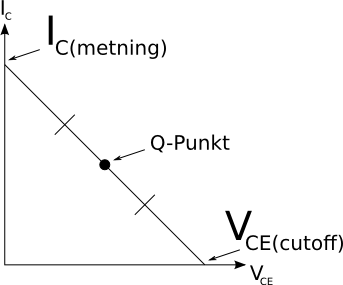
\includegraphics[width=0.5\textwidth]{./img/lastlinje}
\\\\
$$I_{C(metning)} = \frac{V_{RC}}{R_C}$$
$$V_{CE(cutoff)} = V_{cc}$$
Man bruker dette når man velger hvor store motstandere man vil ha.
$$R_C = \frac{V_{CE}}{I_C}$$
